\documentclass[12pt]{beamer}
\usepackage{inputenc}
\usepackage{lmodern}
\usepackage{algorithm,algorithmic}
\usepackage{graphicx}
\usepackage{tikz}
\usepackage{booktabs}
\usepackage{hyperref}
\usetheme{AnnArbor}

\hypersetup{colorlinks,linkcolor={blue},citecolor={blue},urlcolor={red}}

\begin{document}
    \author{Nhóm sinh viên 19CTT2}
    \title{Thuật toán Floyd-Warshall}
    \subtitle{Tìm đường đi ngắn nhất giữa mọi cặp đỉnh}
    %\logo{}
    \institute{fit@hcmus}
    \date{mùa Xuân năm 2021}
    %\subject{}
    %\setbeamercovered{transparent}
    %\setbeamertemplate{navigation symbols}{}
    \begin{frame}[plain]
        \maketitle
    \end{frame}

    \section{Tài liệu tham khảo}
    \begin{frame}[allowframebreaks]
        \frametitle{Tài liệu tham khảo}
        \bibliographystyle{apalike}
        \bibliography{bib/algo}
    \end{frame}

    \begin{frame}
    \frametitle{Nội dung chính}
    \tableofcontents
    \end{frame}

    \section{Giới thiệu}
    \begin{frame}
        \frametitle{Bài toán đường đi ngắn nhất}
        \begin{itemize}
            \item Trong một đồ thị không trọng số, đường đi ngắn nhất giữa 2 đỉnh = $min$(số lượng cạnh phải đi qua).\pause
            \item Trong đồ thị có trọng số, đường đi ngắn nhất là đường đi có tổng trọng số đạt $ min $.\pause
            \item Thuật toán Dijkstra là một thuật toán hiệu quả để giải quyết bài toán đường đi ngắn nhất trên đồ thị có trọng số.\cite{dijkstra1959note}
        \end{itemize}
    \end{frame}

    \begin{frame}[plain]
        \begin{figure}
            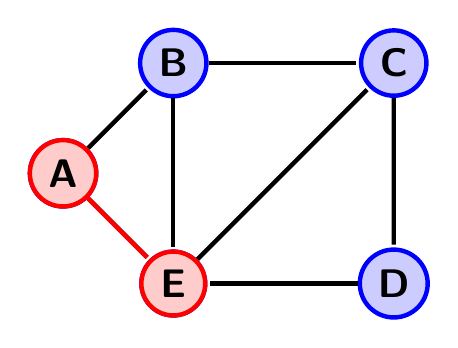
\begin{tikzpicture}[scale=.7,shorten >=1pt, auto, node distance=1.5cm, ultra thick]
            \begin{scope}[every node/.style={circle,draw=blue,fill=blue!20!,font=\sffamily\Large\bfseries}]
            \node (v1) at (-4,0) {A};
            \node (v5) at (-2,-2) {E};
            \node (v2) at (-2,2) {B};
            \node (v3) at (2,2) {C};
            \node (v4) at (2,-2) {D};
            \end{scope}
            \begin{scope}[every edge/.style={draw=black,ultra thick}]
            \draw  (v1) edge (v2);
            \draw  (v1) edge (v5);
            \draw  (v2) edge (v3);
            \draw  (v2) edge (v5);
            \draw  (v3) edge (v4);
            \draw  (v4) edge (v5);
            \draw  (v5) edge (v3);
            \end{scope}
            \begin{scope}[every node/.style={circle,draw=red,fill=red!20!,font=\sffamily\Large\bfseries}]
            \node (v1) at (-4,0) {A};
            \node (v5) at (-2,-2) {E};
            \end{scope}\pause
            \begin{scope}[every edge/.style={draw=red, ultra thick}]
            \draw  (v1) edge (v5);
            \end{scope}
            \end{tikzpicture}
            \caption{Đường đi ngắn nhất từ đỉnh $A$ đến đỉnh $E$ trên đồ thị không trọng số.}
        \end{figure}
    \end{frame}

    \begin{frame}[plain]
        \begin{figure}
        \begin{minipage}{.45\textwidth}
            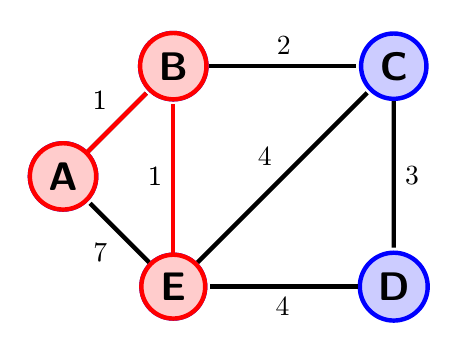
\begin{tikzpicture}[scale=.7,shorten >=1pt, auto, node distance=1.5cm, ultra thick]
            \begin{scope}[every node/.style={circle,draw=blue,fill=blue!20!,font=\sffamily\Large\bfseries}]
            \node (v1) at (-4,0) {A};
            \node (v2) at (-2,2) {B};
            \node (v5) at (-2,-2) {E};
            \node (v3) at (2,2) {C};
            \node (v4) at (2,-2) {D};
            \end{scope}
            \begin{scope}[every edge/.style={draw=black,ultra thick}]
            \draw  (v1) edge node{1} (v2);
            \draw  (v5) edge node{1} (v2);
            \draw  (v2) edge node{2} (v3);
            \draw  (v3) edge node{3} (v4);
            \draw  (v4) edge node{4} (v5);
            \draw  (v5) edge node{7} (v1);
            \draw  (v5) edge node{4} (v3);
            \end{scope}
            \begin{scope}[every node/.style={circle,draw=red,fill=red!20!,font=\sffamily\Large\bfseries}]
            \node (v1) at (-4,0) {A};
            \node (v5) at (-2,-2) {E};
            \end{scope}\pause
            \begin{scope}[every node/.style={circle,draw=red,fill=red!20!,font=\sffamily\Large\bfseries}]
            \node (v2) at (-2,2) {B};
            \end{scope}
            \begin{scope}[every edge/.style={draw=red, ultra thick}]
            \draw  (v1) edge node{1} (v2);
            \draw  (v5) edge node{1} (v2);
            \end{scope}
            \end{tikzpicture}
        \end{minipage}
        \caption{Đường đi ngắn nhất từ đỉnh $A$ đến đỉnh $E$ trên đồ thị mang trọng số.}
        \end{figure}
    \end{frame}

    \begin{frame}
        \frametitle{Cung âm}
        \begin{itemize}
            \item Một cạnh trong đồ thị (có hướng hoặc vô hướng) mang trọng số âm được gọi là \textit{cung âm}.\pause
            \item Một nhược điểm của thuật toán Dijkstra: cho kết quả sai khi đồ thị có cung âm!\pause
            \item Để khắc phục, ta phải sử dụng một thuật toán khác: Bellman-Ford hoặc Floyd-Warshall.
        \end{itemize}
    \end{frame}

    \begin{frame}[t]
        \frametitle{Giới thiệu thuật toán Floyd-Warshall}

        \begin{itemize}
            \item Được phát biểu riêng lẻ bởi Stephen Warshall năm 1959\cite{10.1145/321105.321107} và Robert W. Floyd năm 1962\cite{10.1145/367766.368168}.\pause
            \item Là một thuật toán Quy hoạch động tiêu biểu.\pause
        \end{itemize}

        \begin{minipage}{0.45\textwidth}
        \begin{figure}
            \includegraphics[scale=0.5]{algo/floyd.png}
            \caption{Robert W. Floyd}
        \end{figure}\pause
        \end{minipage}
        \begin{minipage}{0.45\textwidth}
        \begin{figure}
            \includegraphics[scale=2]{algo/warshall.jpg}
            \caption{Stephen Warshall}
        \end{figure}
        \end{minipage}
    \end{frame}

    \section{Ý tưởng}
    \begin{frame}
        \frametitle{Ý tưởng}
        \framesubtitle{Khởi tạo mảng đường đi $F$}
        Xét một đồ thị vô hướng hoặc có hướng.

        Gọi $ F[A][B] $ là độ dài đường đi ngắn nhất từ đỉnh $ A $ đến đỉnh $ B $.\pause
        \begin{itemize}
            \item $F[A][A] = 0$, từ một đỉnh không tốn chi phí để đi đến chính nó.\pause
            \item $F[A][B] = k$, nếu có một cung nối trực tiếp $ A $ và $ B $ mang trọng số $k$.\pause
            \item $F[A][B] = \infty$, nếu không có cung nối $ A $ và $ B $.
        \end{itemize}
    \end{frame}
    \begin{frame}
    \frametitle{Ý tưởng}
    \framesubtitle{Công thức truy hồi}
    $ \centering F[A][B] = min(F[A][K] + F[K][B], F[A][B])$

    với $ K $ là một đỉnh trung gian sao cho tồn tại đường đi từ $ A $ đến $ K $ và từ $ K $ đến $ B $.
    \end{frame}

    \begin{frame}
        \frametitle{Ý tưởng (cont.)}
        \framesubtitle{Truy vết}
        Do thuật toán Floyd-Warshall là một thuật toán quy hoạch động nên ta có thể áp dụng phương pháp truy vết:

        Gọi $T$ là ma trận lưu vết,\pause
        \begin{itemize}
            \item $T[A][A] = A$.\pause
            \item $T[A][B] = B \iff $ có một cung nối $A$ và $B$.\pause
            \item $T[A][B] = T[A][K]\iff$ có một cung nối $A$ và $K$; một cung nối $K$ và $B$.
        \end{itemize}
    \end{frame}

    \begin{frame}
        \frametitle{Ý tưởng}
        \framesubtitle{Minh họa}

        \begin{minipage}{.55\textwidth}
          \begin{figure}
            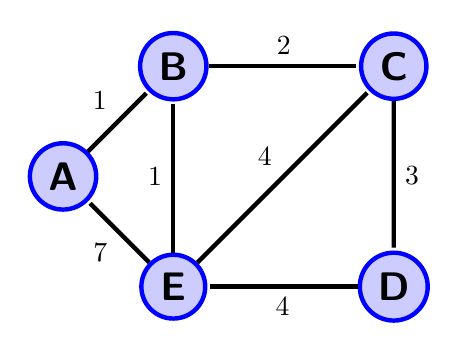
\begin{tikzpicture}[scale=.7,shorten >=1pt, auto, node distance=1.5cm, ultra thick]
            \begin{scope}[every node/.style={circle,draw=blue,fill=blue!20!,font=\sffamily\Large\bfseries}]
            \node (v1) at (-4,0) {A};
            \node (v2) at (-2,2) {B};
            \node (v3) at (2,2) {C};
            \node (v4) at (2,-2) {D};
            \node (v5) at (-2,-2) {E};
            \end{scope}
            \begin{scope}[every edge/.style={draw=black,ultra thick}]
            \draw  (v1) edge node{1} (v2);
            \draw  (v2) edge node{2} (v3);
            \draw  (v3) edge node{3} (v4);
            \draw  (v4) edge node{4} (v5);
            \draw  (v5) edge node{7} (v1);
            \draw  (v5) edge node{1} (v2);
            \draw  (v5) edge node{4} (v3);
            \end{scope}
            \end{tikzpicture}
           \caption{Đồ thị minh họa với $\mathcal{V} = 5, \mathcal{E} = 7$}
          \end{figure}
        \end{minipage}
        \begin{minipage}{.4\textwidth}
            \begin{table}[ht]
                \begin{tabular}[t]{cccccc}
                      & A & B & C & D & E\\
                    \midrule
                    A & 0 & 1 & $\infty$ & $\infty$ & 7\\
                    B & 1 & 0 & 2 & $\infty$ & 1\\
                    C & $\infty$ & 2 & 0 & 3 & 4\\
                    D & $\infty$ & $\infty$ & 3 & 0 & 4\\
                    E & 7 & 1 & 4 & 4 & 0\\
                \end{tabular}
                \caption{Bảng giá trị $F[u][v]$}
            \end{table}
        \end{minipage}
    \end{frame}


    \begin{frame}
        \frametitle{Ý tưởng}
        \framesubtitle{Minh họa (cont.)}

        \begin{minipage}{.55\textwidth}
            \begin{figure}
                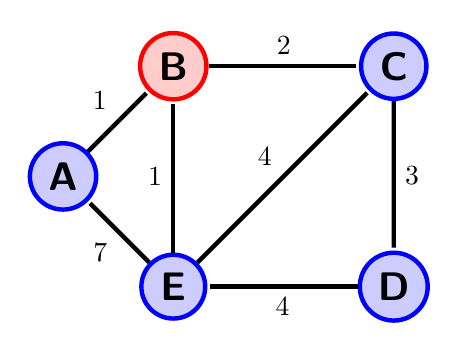
\begin{tikzpicture}[scale=.7,shorten >=1pt, auto, node distance=1.5cm, ultra thick]
                \begin{scope}[every node/.style={circle,draw=blue,fill=blue!20!,font=\sffamily\Large\bfseries}]
                \node (v1) at (-4,0) {A};
                \node (v3) at (2,2) {C};
                \node (v4) at (2,-2) {D};
                \node (v5) at (-2,-2) {E};
                \end{scope}
                \begin{scope}[every node/.style={circle, draw=red,fill=red!20!,font=\sffamily\Large\bfseries}]
                \node (v2) at (-2,2) {B};
                \end{scope}
                \begin{scope}[every edge/.style={draw=black,ultra thick}]
                \draw  (v1) edge node{1} (v2);
                \draw  (v2) edge node{2} (v3);
                \draw  (v3) edge node{3} (v4);
                \draw  (v4) edge node{4} (v5);
                \draw  (v5) edge node{7} (v1);
                \draw  (v5) edge node{1} (v2);
                \draw  (v5) edge node{4} (v3);
                \end{scope}
                \end{tikzpicture}
                \caption{Cập nhật độ dài các cặp cạnh có đỉnh trung gian $B$.}
            \end{figure}
        \end{minipage}
        \begin{minipage}{.4\textwidth}
            \begin{table}[ht]
                \begin{tabular}[t]{cccccc}
                    & A & B & C & D & E\\
                    \midrule
                    A & 0 & 1 & \textcolor{red}{3} & $\infty$ & \textcolor{red}{2}\\
                    B & 1 & 0 & 2 & $\infty$ & 1\\
                    C & \textcolor{red}{3} & 2 & 0 & 3 & \textcolor{red}{3}\\
                    D & $\infty$ & $\infty$ & 3 & 0 & 4\\
                    E & \textcolor{red}{2} & 1 & \textcolor{red}{3} & 4 & 0\\
                \end{tabular}
            \end{table}
        \end{minipage}
    \end{frame}
    \begin{frame}
    \frametitle{Ý tưởng}
    \framesubtitle{Minh họa (cont.)}

    \begin{minipage}{.55\textwidth}
        \begin{figure}
            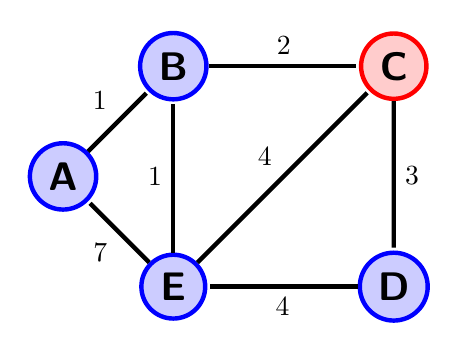
\begin{tikzpicture}[scale=.7,shorten >=1pt, auto, node distance=1.5cm, ultra thick]
            \begin{scope}[every node/.style={circle,draw=blue,fill=blue!20!,font=\sffamily\Large\bfseries}]
            \node (v1) at (-4,0) {A};
            \node (v2) at (-2,2) {B};
            \node (v4) at (2,-2) {D};
            \node (v5) at (-2,-2) {E};
            \end{scope}
            \begin{scope}[every node/.style={circle, draw=red,fill=red!20!,font=\sffamily\Large\bfseries}]
            \node (v3) at (2,2) {C};
            \end{scope}
            \begin{scope}[every edge/.style={draw=black,ultra thick}]
            \draw  (v1) edge node{1} (v2);
            \draw  (v2) edge node{2} (v3);
            \draw  (v3) edge node{3} (v4);
            \draw  (v4) edge node{4} (v5);
            \draw  (v5) edge node{7} (v1);
            \draw  (v5) edge node{1} (v2);
            \draw  (v5) edge node{4} (v3);
            \end{scope}
            \end{tikzpicture}
            \caption{Cập nhật độ dài các cặp cạnh có đỉnh trung gian $C$.}
        \end{figure}
    \end{minipage}
    \begin{minipage}{.4\textwidth}
        \begin{table}[ht]
            \begin{tabular}[t]{cccccc}
                & A & B & C & D & E\\
                \midrule
                A & 0 & 1 & 3 & \textcolor{red}{6} & 2\\
                B & 1 & 0 & 2 & \textcolor{red}{5} & 1\\
                C & 3 & 2 & 0 & 3 & 3\\
                D & \textcolor{red}{6} & \textcolor{red}{5} & 3 & 0 & 4\\
                E & 2 & 1 & 3 & 4 & 0\\
            \end{tabular}
        \end{table}
    \end{minipage}
    \end{frame}

    \begin{frame}
        \frametitle{Ý tưởng (cont.)}
        \framesubtitle{Nhận xét}
        \textbf{Nhận xét}: Gọi $ F $ là ma trận đường đi sau khi đã tính toán bằng thuật toán Floyd-Warshall.\pause
        \begin{itemize}
            \item Thuật toán Floyd-Warshall \textbf{tính toán đường đi giữa tất cả các cặp đỉnh}. Khi cần sử dụng, ta chỉ cần tra $ F $[<đỉnh đi>][<đỉnh đến>] đã tính toán sẵn.\pause
            \item Nếu $F[A][B] = \infty $ thì \textbf{không tồn tại} một đường đi từ đỉnh $A$ đến đỉnh $B$.\pause
            \item Có thể sử dụng thuật Floyd-Warshall để \textbf{nhận biết chu trình âm}: $F[A][B] < 0 \iff $ giữa $ A $ và $ B $ tồn tại một chu trình âm.\footnote{chu trình âm là chu trình có tổng trọng số âm}\cite{gtlt:book}
        \end{itemize}
    \end{frame}

    \section{Cài đặt}
    \begin{frame}
        \frametitle{Cài đặt}
        \framesubtitle{Khởi tạo mảng $F$ lưu đường đi ngắn nhất giữa mọi cặp đỉnh}
        \begin{algorithm}[H]
            \begin{algorithmic}[1]
                \FOR{$i=1$ to $N$}
                \STATE $F[i][i] = 0$
                \ENDFOR
            \end{algorithmic}
            \caption{Khởi tạo đường đi ngắn nhất cho từng đỉnh tới chính nó}
        \end{algorithm}
    \end{frame}
    \begin{frame}
        \frametitle{Cài đặt (cont.)}
        \framesubtitle{Khởi tạo ma trận $F$ lưu đường đi ngắn nhất giữa mọi cặp đỉnh}
        \begin{algorithm}[H]
            \begin{algorithmic}[1]
                \FOR{$i=1$ to $N$}
                \FOR{$j=1$ to $N$}
                \STATE $T[i][j] = j$
                \IF {$i \neq j$}
                \IF {có cung nối $i$ và $j$ mang trọng số $k$}
                \STATE $F[i][j] = k$
                \ELSE
                \STATE $F[i][j] = \infty$
                \ENDIF
                \ENDIF
                \ENDFOR
                \ENDFOR
            \end{algorithmic}
            \caption{Khởi tạo đường đi ban đầu giữa các đỉnh}
        \end{algorithm}
    \end{frame}
    \begin{frame}
        \frametitle{Cài đặt (cont.)}
        \framesubtitle{Tính toán đường đi ngắn nhất giữa các cặp đỉnh}
        \begin{algorithm}[H]
            \begin{algorithmic}[1]
                \FOR{$k=1$ to $N$}
                \FOR{$i=1$ to $N$}
                \FOR{$j=1$ to $N$}
                \IF {$F[i][k] + F[k][j] < F[i][j]$}
                \STATE $F[i][j] = F[i][k] + F[k][j]$
                \STATE $T[i][j] = T[i][k]$
                \ENDIF
                \ENDFOR
                \ENDFOR
                \ENDFOR
            \end{algorithmic}
            \caption{Tính toán đường đi ngắn nhất giữa các cặp đỉnh}
            \label{alg:seq}
        \end{algorithm}
    \end{frame}
    \begin{frame}
        \frametitle{Cài đặt (cont.)}
        \framesubtitle{In ra đường đi ngắn nhất}
        Giả sử ta cần in ra đường đi ngắn nhất từ đỉnh $S$ đến đỉnh $F$:
        \begin{algorithm}[H]
            \begin{algorithmic}[1]
                \WHILE {$S \neq F$}
                \STATE in đỉnh $S$
                \STATE $S = T[S][F]$
                \ENDWHILE
                \STATE in đỉnh $F$
            \end{algorithmic}
            \caption{In đường đi ngắn nhất}
        \end{algorithm}
    \end{frame}
    \begin{frame}
        \Large \centering
        Demo (C++)
    \end{frame}


    \section{Đánh giá}
    \begin{frame}
        \frametitle{Đánh giá}
        \framesubtitle{Độ phức tạp thời gian}
        \begin{itemize}
            \item Độ phức tạp trong trường hợp tốt nhất: $\mathcal{O}(n^3)$
            \item Độ phức tạp trong trường hợp tệ nhất: $\mathcal{O}(n^3)$
            \item Độ phức tạp trung bình: $\mathcal{O}(n^3)$
        \end{itemize}\pause
        \textbf{Nhận xét:} Thuật toán Floyd-Warshall có độ phức tạp khá \textbf{tệ} ($\mathcal{O}(n^3)$ trong hầu hết trường hợp) nhưng độ phức tạp mỗi truy vấn đường đi ngắn nhất sẽ là $\mathcal{O}(1)$.
    \end{frame}

    \begin{frame}
        \frametitle{Đánh giá (cont.)}
        \framesubtitle{Độ phức tạp không gian}
        \begin{itemize}
            \item Độ phức tạp không gian trong trường hợp tốt nhất: $\mathcal{O}(n^2)$
            \item Độ phức tạp không gian trong trường hợp tệ nhất: $\mathcal{O}(n^2)$
            \item Độ phức tạp không gian trung bình: $\mathcal{O}(n^2)$
        \end{itemize}
    \end{frame}

    \section{Cải tiến \& ứng dụng}
    \begin{frame}
        \frametitle{Cải tiến}
        \begin{itemize}
        \item Một cải tiến được H.Grag và P.Rawat đưa ra năm 2012\cite{improve:article}, theo đó làm giảm độ phức tạp xuống một cách \textbf{đáng kể}, từ $\mathcal{O}(n^3)$ xuống còn $\mathcal{O}(n^{3 - \epsilon})$.
        \item Cách cài đặt được để dành cho bạn đọc luyện tập.
        \end{itemize}
    \end{frame}

    \begin{frame}
        \frametitle{Ứng dụng}
        Trong lý thuyết đồ thị:
        \begin{itemize}
            \item Phát hiện chu trình âm trong đồ thị.
            \item Tìm đường đi ngắn nhất giữa mọi cặp đỉnh trên đồ thị.
        \end{itemize}\pause
        Trong thực tế:
        \begin{itemize}
            \item Xây dựng mạng lưới giao thông tối ưu ở các thành phố lớn.
            \item Tính toán bao đóng truyền ứng \textit{(Transitive Closure)}
            \item Dùng nhiều trong việc định tuyến mạng máy tính.
        \end{itemize}
    \end{frame}

    \begin{frame}
        \frametitle{Tổng kết}
        \begin{itemize}
            \item Thuật toán Floyd-Warshall rất dễ cài đặt.\pause
            \item Với độ phức tạp trung bình và tệ nhất đều là $\mathcal{O}(n^3)$, thuật toán Floyd-Warshall nên được cân nhắc khi sử dụng trong các bài toán đồ thị.\pause
            \item Có nhiều ứng dụng trong lý thuyết đồ thị, toán học và thực tế.
        \end{itemize}
    \end{frame}

    \begin{frame}
        \Large \centering
        The End!
    \end{frame}

    \section{Credit}
    \begin{frame}
        \frametitle{Credit}
        \centering
        \begin{table}[H]
            \begin{tabular}[t]{ll}
                \toprule
                \multicolumn{2}{c}{Nhóm sinh viên thực hiện} \\
                \midrule
                Ngô Đặng Gia Lâm & 19120268\\
                Trần Hoàng Quân & 19120338\\
                Huỳnh Tấn Thọ & 19120383\\
                Lâm Hải Triều & 19120407\\
                Sử Nhật Đăng & 19120469\\
                \bottomrule
            \end{tabular}
        \end{table}
        Mùa Xuân năm 2021.
    \end{frame}
\end{document}